\documentclass[12pt,a4paper]{article}
\usepackage{cmap} % Makes the PDF copiable. See http://tex.stackexchange.com/a/64198/25761
\usepackage[T1]{fontenc}
\usepackage[brazil]{babel}
\usepackage[utf8]{inputenc}
\usepackage{amsmath}
\usepackage{amsfonts}
\usepackage{amssymb}
\usepackage{amsthm}
\usepackage{textcomp} % \degree
\usepackage{gensymb} % \degree
\usepackage[usenames,svgnames,dvipsnames]{xcolor}
\usepackage{hyperref}
\usepackage{multicol}
\usepackage{graphicx}
\usepackage{systeme}
\usepackage[margin=2cm]{geometry}

\hypersetup{
    colorlinks = true,
    allcolors = {blue}
}

\newcommand{\vect}[1]{\overrightarrow{#1}}
\newcommand{\norm}[1]{\left|\left|{#1}\right|\right|}

\newcommand*\tipo{PROVA IV}
\newcommand*\turma{TURMA E}
\newcommand*\disciplina{GAN0001}
\newcommand*\nome{GEOMETRIA ANALÍTICA}
\newcommand*\eu{Helder G. G. de Lima}
\newcommand*\data{30/06/2015}

\author{\eu}
\title{\tipo - \disciplina}
\date{\data}

\begin{document}
\thispagestyle{empty}
\newgeometry{margin=2cm,bottom=0.5cm}
\begin{center}

\includegraphics{udesc_joinville_cabecalho.pdf}
\\ Prof. \eu\footnote{
Este é um material de acesso livre distribuído sob os termos da licença \href{https://creativecommons.org/licenses/by-sa/4.0/deed.pt_BR}{Creative Commons BY-SA 4.0}.}

\noindent\begin{tabular}{l c c r}
  \textbf{\disciplina}
& \textbf{\tipo}
& \textbf{\data}
& \textbf{\turma}
\end{tabular}\vspace{-0.3cm}
\noindent\rule{17cm}{0.01cm}
\end{center}

\noindent Nome do(a) aluno(a): \rule{13cm}{0.01cm}

%\section*{Instruções}
{\footnotesize
\begin{enumerate}
\renewcommand{\theenumi}{\Roman{enumi}}
\item Identifique-se em todas as folhas.
\item Mantenha o celular e os demais equipamentos eletrônicos desligados durante a prova.
\item Justifique cada resposta com cálculos ou argumentos baseados na teoria estudada.
\item Escolha \textsc{\textbf{uma}} questão para \textsc{\textbf{não}} fazer (ela não será corrigida): \rule{3cm}{0.01cm}
\end{enumerate}
}

\noindent\rule{17cm}{0.01cm}
%\section*{Questões}

\begin{enumerate}
\item (2,0 pontos) A equação $r = 3-\cos( \theta )$ representa uma curva em coordenadas polares.
\begin{enumerate}
\item (0,5 pontos) Explique se há simetria em relação a algum eixo e em relação à origem
\item (0,5 pontos) Calcule as coordenadas polares de 5 pontos pertencentes à curva
\item (1,0 pontos) Esboce o gráfico (utilize o verso desta folha)
\end{enumerate}

\item (2,0 pontos) Se $r = \dfrac{10}{1+\cos(\theta)}$ é a equação de uma parábola em coordenadas polares, qual é a equação em coordenadas cartesianas? E as coordenadas \textbf{polares} do vértice?

\item Seja $r \operatorname{sen}(\phi) = 7$ a equação de uma superfície em coordenadas \textbf{esféricas}.
\begin{enumerate}
\item (1,0 pontos) Qual é a equação da superfície em coordenadas cartesianas?
\item (0,7 pontos) Quais são os pontos de interseção com os eixos coordenados?
\item (0,3 pontos) Qual o nome da superfície?
\end{enumerate}

\item (2,0 pontos) Forneça a equação, o nome e um esboço da quádrica formada pelos pontos $P = (x, y, z)$ cuja distância ao ponto $Q=(0, 0, 2)$ é igual à distância ao plano $xOy$.

\item Seja $(z-2)^2 = (2-r)(2+r)$ a equação de uma superfície em coordenadas \textbf{cilíndricas}.
\begin{enumerate}
\item (0,5 pontos) Qual é a equação da superfície em coordenadas cartesianas?
\item (0,5 pontos) Quais são as interseções com os planos coordenados?
\item (1,0 pontos) Nomeie e esboce a superfície, indicando pontos e curvas relevantes.
\end{enumerate}

\item Considere a superfície $\dfrac{(x-3)^2}{9} - (y-5)^2 - \dfrac{(z-2)^2}{4} = 1$.
\begin{enumerate}
\item (0,8 pontos) Descreva (por nome e equação) a interseção com o plano $y = 6$.
\item (1,2 pontos) Para que valores de $k \in \mathbb{R}$ \textbf{não há} interseção com o plano $x = k$?
\end{enumerate}
\end{enumerate}

\section*{Lembrete}
\begin{itemize}\footnotesize
\begin{multicols}{3}
\item
$\begin{cases}
x & = r \cos(\theta)\\
y & = r \operatorname{sen}(\theta)\\
\end{cases}$
\item
$\begin{cases}
x & = r \operatorname{sen}(\phi) \cos(\theta)\\
y & = r \operatorname{sen}(\phi) \operatorname{sen}(\theta)\\
z & = r \cos(\phi)
\end{cases}$
\item
$\begin{cases}
x & = r \cos(\theta)\\
y & = r \operatorname{sen}(\theta)\\
z & = z
\end{cases}$
\end{multicols}
\end{itemize}

\newpage
\restoregeometry
%\begin{enumerate}
\begin{multicols}{2}
%\renewcommand{\theenumi}{\alph{enumi}}%
%\item
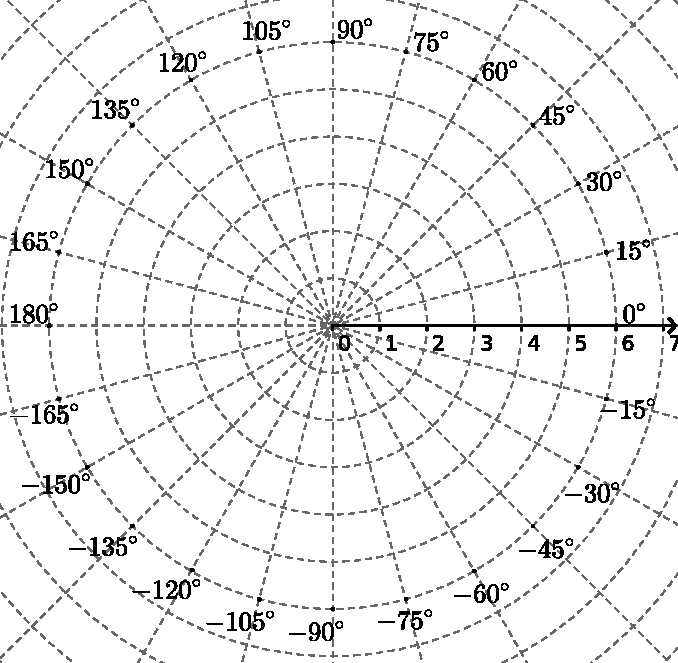
\includegraphics[width=7.5cm]{img/prova-4-civ-malha-1}
\vspace{2em}
%\item
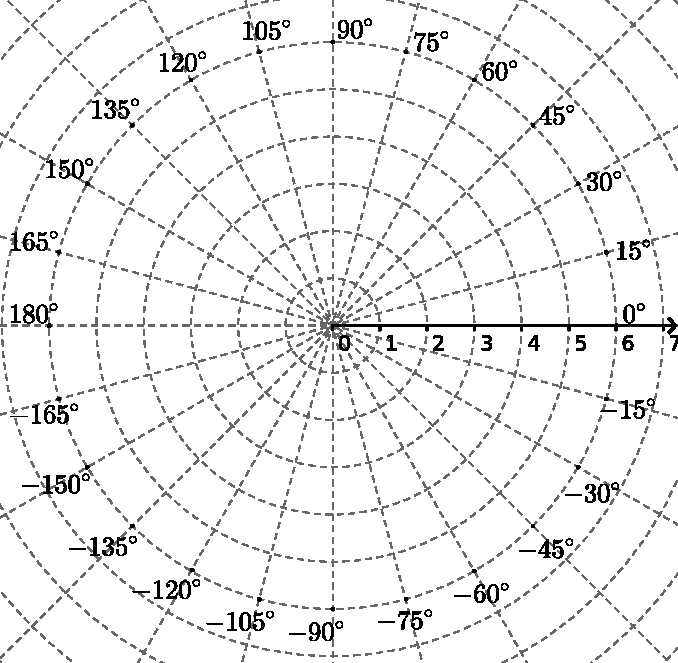
\includegraphics[width=7.5cm]{img/prova-4-civ-malha-1}
\end{multicols}
%\item

\includegraphics[width=16cm]{img/prova-4-civ-malha-2}

\vspace{2em}

\includegraphics[width=16cm]{img/prova-4-civ-malha-2}
%\end{enumerate}

%\newpage
%\section*{Respostas e observações}
%\begin{enumerate}
%\item \textit{\fixme}
%\end{enumerate}

\end{document}
